\documentclass[twoside,11pt]{report}

\usepackage{fontspec}
\setmainfont{Palatino}
% \usepackage{url}
\usepackage{hyperref}
\usepackage{graphicx}
\usepackage{enumitem}
\usepackage[table]{xcolor}
\usepackage{color}

\usepackage{amsmath}
\usepackage{amsfonts}
\usepackage{multirow}
\usepackage{caption}
\usepackage{subcaption}
\DeclareMathOperator*{\argmax}{arg\,max}

\usepackage{natbib}
\bibpunct[; ]{(}{)}{,}{a}{}{;}

\usepackage{graphicx}
\usepackage{fancyvrb}

\usepackage{geometry}
\geometry{
  top=1.0in,
  inner=1.0in,
  outer=1.0in,
  bottom=1.0in,
  headheight=3ex,
  headsep=2ex,
}
\usepackage{fancyhdr}
\pagestyle{fancyplain}

\lhead{}
\chead{\fancyplain{}{A Research Agenda for Historical and Multilingual Optical Character Recognition}}
\rhead{}

\newcounter{reccounter}
\renewcommand{\thereccounter}{\arabic{reccounter}}
\newcommand{\recommend}[2]{\refstepcounter{reccounter}%
  \label{rec:#1}%
  \subsection{\#\thereccounter. #2}%
  \label{sec:rec-#1}}

\newcounter{appcounter}
\renewcommand{\theappcounter}{\Alph{appcounter}}
\renewcommand{\appendix}[2]{\refstepcounter{appcounter}%
  \label{app:#1}%
  \section{Appendix~\theappcounter: #2}%
  \label{sec:app-#1}}

\renewcommand{\bibname}{References}
\usepackage[numbib]{tocbibind}

\setcounter{secnumdepth}{-1}

\usepackage{eso-pic}
\newcommand\BackgroundPic{%
\put(0,0){%
\parbox[b][\paperheight]{\paperwidth}{%
\vfill
\centering
\includegraphics[width=\paperwidth]{VA013RN-0014-mask.png}%
\vfill
}}}

\title{\Huge A Research Agenda for \\ Historical and Multilingual \\ Optical Character Recognition}

\author{\huge David A. Smith \and \huge Ryan Cordell}

\date{\centering \vspace{0.2in} 
\includegraphics[width=5in]{northeastern.png} \vspace{0.5in} \\
  
\includegraphics{nulab.png} \\
  \vspace{0.2in} \centering \huge with the support of \\ \vspace{0.1in}
  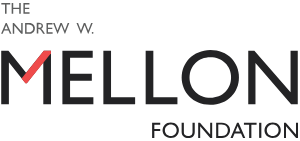
\includegraphics{mellon.png}}

\begin{document}
\AddToShipoutPicture*{\BackgroundPic}

\maketitle

\copyright 2018 David A. Smith and Ryan Cordell

Image credits

The image of Venetus A (Marciana 822 = Graecus Z. 454) is derived from an original that is \copyright 2007, Biblioteca Nazionale Marciana, Venezia, Italia. The derivative image is \copyright 2010, Center for Hellenic Studies. All original and derivative images are licensed under the Creative Commons Attribution-Noncommercial-Share Alike 3.0 License. The CHS/Marciana Imaging Project was directed by David Jacobs of the British Library.

\tableofcontents

\chapter{Summary}
\label{sec:summary}

Scholars across every research discipline depend on text. Scholars in most humanities and social sciences disciplines, for example, spend a significant amount of the research time reading, analyzing, grouping, and comparing large bodies of text, whether those be from newspapers or books or historic documents. Today, of course, much of this text lives online in digital libraries of one sort or another. Most modern text is ``born digital'' meaning that it was originally created using a computer. So when a scholar wishes to search a recent edition of the New York Times, she doesn't need to worry about the text containing rampant misspellings. But what if a historian wishes to search issues from the Civil War era of the 1860s? While those issues have indeed been digitized---along with millions of other print and manuscript pages---the actual text is riddled with so many misspelled words that standard searching or computational text analysis become impractical. The proportion of erroneous words in nineteenth-century newspapers in English can exceed 40\%; error rates can be even higher for other languages and earlier periods. These transcription errors are due to the difficulties in converting the scanned images of each page into actual computer text---what is commonly called Optical Character Recognition (OCR). This report is about methods to improve OCR for print texts and manuscripts to allow for new kinds of research on previously inaccessible sources.

\section{Who is the intended audience for this report?}

This report is addressed to several audiences:
\begin{itemize}

\item Computer scientists, library and information scientists, and other scholars researching new methods in computer vision, natural language processing, information retrieval, machine learning, and related fields. Such individuals are in a position to tackle the kind of research this report identifies as critical to improving the overall quality of OCR'd texts.

\item Commercial and nonprofit developers and providers of OCR technologies and services and of OCR'd texts.

\item Funders in the humanities, social sciences, computer sciences, information sciences, and cultural heritage who are in a position to support the recommendations in this report. Such investments will not only ultimately lead to new research insights across disciplinary domains, but will also make the research process more efficient and cost-effective, as scholars will be spending less time trying to overcome problems associated with poor quality OCR'd text.

\item Scholars across academic disciplines---most notably the humanities and social sciences---who are doing computational text-based research. This includes not only scholars who do this kind of work on a regular basis (e.g., computational linguists), but historians, philosophers, political scientists, literary scholars, or anyone whose work searches, compares, and groups textual data. These scholars may benefit from better tools to understand the results from OCR'd collections they are already search every day, or they may wish to use OCR to expand the corpora and languages they currently work with.

\item Senior leaders in libraries and archives that contain large digital collections of text, including newspapers, books, journals, manuscripts, etc. Senior leaders are in a position to make funding available to put best practices in place to ensure the highest-quality OCR methods are not only used initially, but re-applied as OCR technology improves.

\item Scholarly societies and advocacy groups such as the Digital Library Federation, the Council on Library and Information Resources, the Association for Research Libraries, the Modern Language Association, the American Historical Association, the Association for Computers and the Humanities, the Association of Digital Humanities Organizations, or the Text Encoding Initiative.

\end{itemize}

\section{What are the goals of this report?}

This report emerges from conversations among staff at the Andrew W. Mellon Foundation, the National Endowment for the Humanities, and the Library of Congress. Both NEH and Mellon staff have funded many projects over the years whose directors have reported back that the progress of their work was stymied by poor quality OCR. In some cases, this meant a huge delay in the project as text had to be manually cleaned. In other cases, it meant using entirely different text corpora simply to avoid poor OCR. The Library of Congress, as a major holder of digital text libraries, such as the Chronicling America newspaper collection, noted that while OCR technology may be slowly improving, libraries weren't necessarily aware of those improvements or had the ability to easily re-OCR older collections to improve their quality.

Emerging from these conversations was a grant from the Mellon Foundation to Northeastern University's NULab for Texts, Maps, and Networks to perform an in-depth field study to help put together a research agency for next steps improving OCR. This is the final report of that study and aims to put together a roadmap for next steps.

\section{What does this report recommend, in brief?}

We submit the following nine recommendations, addressed to the various stakeholders above, for improving historical and multilingual OCR over the next five to ten years. We will expand on each of the recommendations later in the report.
\begin{enumerate}

\item \hyperref[sec:rec-stats]{\textbf{Improve statistical analysis of OCR output}}

\textbf{Addressed to:} Researchers in natural language processing and information retrieval; curators of large collections of OCR transcripts; scholars using IR and text mining technologies in their research; funders interested in conducting and publishing digital scholarship with OCR'd texts and in building language technologies to work with noisy input.

\textbf{Goals:} Researchers should develop and distribute tools for training and adapting OCR post-correction models; curators of large collections (e.g., Chronicling America or the HathiTrust) should deploy post-correction models in large repositories of OCR transcripts while preserving existing data; researchers should survey and perform quantitative evaluations of the effect of OCR error on commonly used text-analysis methods, as well as qualitative descriptions of the effects of word error rates of, e.g., 2\%, 10\%, and 20\%; researchers should improve methods for error estimation and statistical communication about the distribution of errors and their effects.

\item \hyperref[sec:rec-layout]{\textbf{Formulate standards for annotation and evaluation of document layout}}

\textbf{Addressed to:} Researchers in computer vision, book history, and bibliography; organizers and sponsors of workshops; standards committees; funders of digital humanities and bibliography (e.g., the Mellon Foundation or the NEH) and/or computer vision and machine learning (e.g, the NSF or DFG).

\textbf{Goals:} Disciplinary societies, conferences, workshops, and standards committees should convene humanists working on transcription and bibliographic analysis with computer vision and OCR researchers to formulate standards for ground-truth annotation for, and evaluation of, document layout analysis; standards committees, such as ALTO, should include book historians and other relevant scholars in discussions on encoding layout; builders of OCR systems and scholars working on transcriptions and editions should annotate data according to these standards to encourage research on layout analysis and computational bibliography.

\item \hyperref[sec:rec-editions]{\textbf{Exploit existing digital editions for training and test data}}

\textbf{Addressed to:} Scholars producing digital editions; NLP researchers; funders in language technologies, library and information science, and the humanities.

\textbf{Goals:} Starting with existing catalogs of digital editions, researchers should collect manual transcriptions, images, and baseline OCR transcripts with page coordinates; researchers should align existing manual transcriptions with baseline OCR output linked to page images; OCR researchers and textual scholars should harmonize transcription standards for consistent training and evaluation.

\item \hyperref[sec:rec-contribution]{\textbf{Develop a reusable contribution system for OCR ground truth}}

\textbf{Addressed to:} Managers of large digitization projects; experts in crowdsourcing, citizen scholarship, and public humanities; teachers of documentary editing; funders in museum and library science and in the humanities.

\textbf{Goals:} Developers associated with cultural heritage institutions and other public humanities organizations, assisted by experts in crowdsourcing and citizen scholarship, should build and maintain reusable tools and formats for creating transcriptions linked to images; tools should support both casual crowdsourcing and production of machine-readable editions as part of humanities education; standards would encourage projects to provide data in a form useful for OCR training.

\item \hyperref[sec:rec-adaptation]{\textbf{Develop model adaptation and search for comparable training sets}}

\textbf{Addressed to:} Machine-learning researchers; managers of large digitization projects; funders interested in supporting efficient large-scale digitization and in domain adaptation for machine learning.

\textbf{Goals:} Researchers should develop offline training and online adaptation methods to exploit existing annotated data; managers of large digitization projects should prioritize collection of training data by measuring performance on the collection as a whole.

\item \hyperref[sec:rec-diverse]{\textbf{Train and test OCR on linguistically diverse texts}}

\textbf{Addressed to:} NLP and OCR researchers and system developers; funders interested in language technologies for low-resource languages and code-switching and in digitization of underserved historical languages.

\textbf{Goals:} Create datasets with significant language variation and mixtures of languages and scripts; build structured models to leverage sparse data; experiment with precision-recall tradeoffs for rare, embedded languages.

\item \hyperref[sec:rec-institutes]{\textbf{Convene OCR Institutes in critical research areas}}

\textbf{Addressed to:} Libraries and other centers for mass digitization; researchers; funders interested in catalyzing progress on OCR for a particular language or domain.

\textbf{Goals:} Funders should convene an OCR Institutes Board to identify potential humanities domains, as well as potential participants, to form OCR Institute(s) that will focus on advancing OCR rapidly for a given domain. Grants should be developed to fund OCR Institutes that will offer grants for concerted, collaborative research in identified domains; transcribe sufficient documents for training; and train specialized domain OCR models.

\item \hyperref[sec:rec-assessment]{\textbf{Create an OCR assessment toolkit for cultural heritage institutions}}

\textbf{Addressed to:} Libraries and other curators of repositories of OCR'd documents; funders looking to improve the efficiency and effectiveness of digitization programs in cultural heritage institutions.

\textbf{Goals:} Provide funding to a well-known digital library organization (e.g. DLF, CLIR, or ARL) or research library, to undertake the creation of an OCR Assessment Toolkit to help cultural heritage institutions determine when collections need to be re-OCR'd. This creation will involve surveying cultural heritage institutions about current OCR evaluation practices; identifying best practices, developing procedures for technical and financial assessment of re-OCRing existing collections, and determining the desirability and feasibility of automating such evaluation.

\item \hyperref[sec:rec-bureau]{\textbf{Establish an ``OCR Service Bureau''}}

\textbf{Addressed to:} Universities; scholarly societies and other non-profit organizations and consortia; funders interested in sustaining historical and multilingual OCR in cultural heritage institutions.

\textbf{Goals:} Funders should recruit library and information science professionals to conduct a formal study toward the establishment of an OCR Service Bureau. This Bureau, hosted by a research library or established digital library organization, would provide expertise and facilitate collaborations among researchers, libraries, and enterprises; host training and evaluation data; and manage computing resources. This initial study should outline possible economic organizational, and governance models for such a Bureau, including a survey of possible managing organizations.

\end{enumerate}

\chapter{The Full Report}

\section{Introduction}

Creating copies and editions of texts has held a central place in the humanities ever since the rise of self-conscious humanistic study seven centuries ago. Creating digital editions likewise forms an important strand in the digital humanities, as in the development of the Text Encoding Initiative (TEI) and the many digital scholarly editions created to its standards. Large-scale scanning projects by commercial, government, and academic entities have typically been thought of as entirely distinct from carefully curated editions and archives, but they have nonetheless greatly expanded access to digital facsimiles and also, through the application of optical character recognition (OCR) technologies, to machine-readable ``editions'' of varying quality. There remains, however, a dearth of interactions among the communities of practice undertaking mass digitization projects, researching and developing OCR systems, or conducting humanities research using OCR'd collections. This report surveys research across the humanities and interpretative social sciences, computer science, library and information science, and business in order to articulate common challenges across these communities of practice and propose collaborative avenues for future research. The proposals we outline have the potential to move the state of the field forward across domains, benefitting a range of researchers, students, and general users of large-scale OCR collections.

\subsection{OCR in the Humanities}

The influence of OCR pervades contemporary humanities research and teaching. Most scholars pay OCR little mind---if they are even aware of it---because corpus analysis seems the province of a small subset of researchers. As Ted Underwood \citeyearpar[p.~64]{Underwood:2014ep} reminds us, however, ``[a]lgorithmic mining of large electronic databases has been quietly central to the humanities for two decades. We call this practice `search,' but `search' is a deceptively modest name for a complex technology that has come to play an evidentiary role in scholarship.'' Researchers and students increasingly rely on databases of digitized historical materials in conducting research, for reasons of geographic or economic access, but also for reasons of preservation, as libraries increasingly restrict physical access to fragile materials after digitization. As a result, researchers and students alike rely on search in OCR collections, often unwittingly. The predominant public interfaces of large-scale archives focus on page images, seeking to present the digitized object as a facsimile of its original, while scholars often cite historical materials directly, even when they were accessed through a digitized edition. Taken together, these practices make it easy to forget that we are all engaged in relatively sophisticated modes of machine reading each time we use a digital archive. Scholars sometimes invoke the OCR of these collections in warnings, as when Andrew Stauffer \citeyearpar{stauffer12:_ninet_centur_archiv_digit_age} cautions, ``Algorithmic searching and text mining'' rely ``almost exclusively on the verbal content of idealized models of nineteenth-century printed materials, models that are themselves vitiated by numerous localized errors in character recognition.''

Such critiques have spurred notable attempts to correct errorful OCR in large scale digitization projects. Bonnie Mak \citeyearpar{mak14:_archaeol_digit} notes that since 1999 the Text Creation Partnership (TCP) has mobilized ``legions of outsourced `vendors' who have keyboarded and tagged over 40,000 early English texts'' in EEBO, as well as another 8,000 for Gale Cengage's Eighteenth-Century Collections Online (ECCO) and Readex's Evans Early American Imprints (Evans-TCP). The Australian Newspaper Digitization Program, the results of which are available through the National Library of Australia's Trove portal, invested significant money in ``manually correcting the titles, subtitles, and first four lines of article text'' over 21 million newspaper pages (as of July 2016), mostly through low-cost, offshore editing services \citep{bode16:_thous_titles_author}. In addition, Trove's interface allows users to manually correct the archive's text data, so that by July 2013, ``more than 100 million lines of text'' had been corrected through ``crowd-sourced effort'' \citep{ayres13:_singin_supper}.  Even so, the majority of Trove's OCR'd text remains uncorrected, as 100 million hand-corrected lines constitute only a small percentage of the total lines across 21 million newspaper pages. Most historical book and newspaper archives have deemed correction of articles too time consuming and costly; therefore, the bulk of keyword search within large scale archives, whether open-access or commercially licensed, depends on the errorful output of OCR.

In large part due to these OCR issues, much computational research in the humanities has restricted itself to small, ``cleaner'' corpora such as Project Gutenberg, EEBO-TCP, the Wright American Fiction collection, the Chadwick-Healey British novels collection, or corpora custom-built for particular studies. The University of Richmond's groundbreaking ``Mining the Dispatch'' project (\url{http://dsl.richmond.edu/dispatch/}), for instance, bases its topic models not on the Chronicling America digitization of the Richmond \emph{Daily Dispatch}, but instead on a hand-transcribed subset of the Daily Dispatch. While that project revealed new insights about this important Civil War era newspaper, its methods could not be easily expanded across the much larger Chronicling America collection or its findings compared against the many other newspapers with only OCR transcriptions.

Too often, discussions of OCR quality in digital humanities (and adjacent fields) begin and end with frustration over its imperfections. There have been few efforts to think systematically or strategically about the problems of errorful OCR or to think creatively about what kinds of research are possible within our current paradigm. On both sides of the OCR question we might diagnose failures of imagination that stymie productive conversation about the past, present, and future of large-scale humanistic data.

We can point to a handful of researchers working with errorful OCR data from HathiTrust, such as more recent work by the Stanford Literary Lab, cultural analytics research by scholars such as Ted Underwood and Andrew Piper, or the TOME (Interactive Topic Model and Metadata visualization) tool developed by Lauren Klein and Jacob Eisenstein. While these projects have amply demonstrated that meaningful patterns can be surfaced even from errorful text data, they too largely decenter their discussions of OCR itself to focus on their results aside from OCR errors. Two projects at Northeastern have addressed OCR errors, and the mitigation of their effects, more directly as part of their broader research: the Viral Texts Project (\url{http://viraltexts.org}), for instance, has employed weighted alignment algorithms that can identify duplicate content---such as reprinted articles---in OCR with high rates of transcription error. Another Northeastern researcher, historian Benjamin Schmidt, has conducted experiments showing that patterns of OCR errors can point to significant features of scanned books, such as the presence of sideways printed charts or significant use of non-Western characters.

We believe similarly experimental approaches to the errorful OCR archive could bear much fruit for humanities researchers, if we can move beyond reductive thinking about ``clean transcriptions'' and ``dirty OCR.'' Bringing researchers together with those who create both OCR algorithms and OCR-depen\-dent archives will allow us to broaden conversations about what changes in text data are necessary for future humanities research and how OCR research might advance those goals within realistic paradigms of labor, funding, and technology.

Most OCR research and systems, meanwhile, have developed without reference to applications in the humanities and have focused on modern, Latin-script documents. While we will not survey the entire field here, we will note some exceptions to this trend and some current developments that show promise for fruitful collaboration between OCR and humanities researchers.

While large-scale scanning projects have generally used off-the-shelf OCR products, several researchers on a smaller scale have found that domain-specific training and modeling provide significant gains in accuracy. The availability of open-source systems can give  scholars of particular languages the ability, though not always the computing and human resources, to build better systems. Bruce Robertson and colleagues have achieved significant improvements in OCR'ing ancient Greek using publisher-specific training sets and system combination.\footnote{\url{http://heml.mta.ca/lace/}}  Uwe Springmann and Anke Lüdeling (2016) found that, for historical German herbal manuals printed between 1487 and 1870, training on diplomatic transcriptions with matched typefaces achieved over 99\% character accuracy. More encouragingly, even training on different historical typefaces could achieve character accuracies above 90\%. That work showed what could be done by retraining existing models. Dan Garrette and colleagues (2015) built an unsupervised model to infer image and language models for historical texts mixing several languages.

Beyond these humanities-specific applications, the overall landscape of OCR research has shifted significantly in the last decade. OCR systems in the past often involved a pipeline of page layout analysis that involved splitting lines, words, and even characters into separate image patches, which would then be classified. With those pipelines, connected scripts such as Arabic or even historically common ligatures in Latin script would present fundamentally different problems from recognizing cleanly separable characters. More recently, most state-of-the-art OCR systems have adopted neural network models with recurrent and convolutional architectures to transcribe entire lines of text at once.\footnote{Many systems now use these architectures. For applications to historical and multilingual scripts in particular, see, e.g., Breuel et al. (2013) and Kiessling et al. (2017).}  These systems, therefore, exhibit much less of a gap between separated and connected scripts---or indeed, between print and manuscript. We expect, therefore, that the problems of historical and multilingual OCR will find a receptive audience in the OCR research community.

\section{Scope of this Report}

This report focuses on optical character recognition of print and manuscript images in a range of languages and scripts, and from a wide range of historical periods. We discuss research that seeks to automatically recognize characters within such documents and output machine-readable text data. There are many related issues that arose in our surveys, interviews, and workshops that deserve closer attention. We will provide an overview of some of these very briefly in the paragraphs below as they pertain to our discussion of OCR, but full studies and discussions of them remain outside the scope of this report.

\subsection{Related Issues}

Survey respondents and interviewees often discussed the poor image quality of digitized documents. This poor quality stems from a range of historical reasons related to the source materials or the digitization process. In some cases materials were digitized using early digital imaging equipment that could not scan with the resolution researchers would expect today. Relatedly, some materials were digitized to standards that would not meet current benchmarks, either because they were digitized before those standards were developed or because they were digitized by organizations or individuals unfamiliar with existing standards. Finally, some digitized materials are of poor quality because their source media---particularly microfilm, which is, for example, often the source for digitized newspaper collections---was itself of poor quality. The quality of source images certainly influences the reliability of OCR output, and in general we find that the earliest digitization projects' OCR is less reliable than that of more recent efforts, even within a given collection. In the Library of Congress' Chronicling America collection of historical newspapers, for instance, those newspapers digitized during the first grant cycles (2005, 2007) tend to present poorer OCR than more recent additions to the collection, so that a paper like the \emph{New York Tribune}---to cite only one, though a prominent, example---is substantially less reliable than many other papers in the collection. Reimaging such collections would do much to improve the resulting OCR. In this report, however, we focus on what can be done to improve OCR without entirely reimaging large-scale collections, which would require much greater investments of time, resources, and physical handling of materials than the potentially more scalable process of re-OCRing existing image collections. Also, as OCR technology improves, marginal images, such as those taken by users with personal camera phones, might rise above the threshold of usefulness. In the end, some collections might still require re-imaging, but we will not make such recommendations here.

We also had discussions about transcribing text and closely-aligned graphical elements in documents such as figures and maps. In the latter case, for instance, existing OCR might recognize the text in maps' legends and related metadata, but not the text within the image, including text in multiple alignments that, for instance, follow drawn geographic features. Nor does current OCR technology do a sufficient job of aligning recognized text with graphic elements in images and maps. Relatedly, we learned of research that seeks to identify unique textual elements such as mathematical and musical notation. Each of these tasks addresses an urgent need for particular research communities, and we can imagine future attention to these areas would prove a natural outgrowth of the immediate recommendations we will make in this report. In this report, however, we will not focus on these approaches in favor of more broad-based recommendations for the improvement of text collections.

\section{Report Research Methods}

This report synthesizes primary literature and practitioner research conducted between the fall of 2017 and the fall of 2018. Throughout all of these activities, we drew on expertise across many communities concerned with OCR of historical documents. These included humanities scholars conducting research using OCR'd collections; librarians and information scientists creating and maintaining OCR collections; as well as computer scientists researching new methods for OCR, both in the academy and in private enterprise.

The first phase of our research was two-pronged, comprising interviews with pre-identified researchers and a broader survey distributed across the study's identified scholarly communities. Drawing on our own understanding of the state of the field in our target communities, we identified a set of individuals (or research groups) and conducted half-hour interviews to better understand their work, their senses of the current state of OCR, as well as the areas they believe to hold the greatest potential for future research. See Appendix~\ref{app:questions} for the list of questions with which we began these interviews, though we often adjusted these prompts as interviews progressed in order to follow individuals' ideas and insights. We will provide access to our notes on these interviews for research purposes upon request.

Second, we created a survey to gather feedback from a wider range of researchers and users invested in our report's questions. The survey questions can be found in Appendix~\ref{app:survey}, but the survey is no longer active. We distributed the survey to a range of academic listservs in humanities fields, digital humanities, library and information sciences, and computer science, and promoted  the survey on social media. Sixty-two people responded to the survey, and their answers proved valuable both in expanding our ideas about the major issues at stake in OCR research and for pointing us to research of which we were unaware. We followed up and conducted formal interviews with several survey participants whose answers we found particularly enlightening. A spreadsheet of the anonymized survey responses can be found at

\url{https://docs.google.com/spreadsheets/d/1_qj-wxXYV0ybVfmR-SS3QzsLplPXGn3XM2pmPSbwbIM/edit?usp=sharing}

Following the initial interviews and survey, we grouped interviewees into five working groups, organized (roughly) around the most prominent shared concerns raised during our initial interviews. The primary challenges facing researchers were clearly articulated during our initial interviews, and so these groups were charged with looking toward the future. Each group began their conversation considering the question: ``given adequate time, attention, and funding, what innovation(s) in OCR would most significantly move research forward in your discipline?''  The point of these working groups was to move beyond listing challenges for historical and multilingual OCR and begin outlining potential solutions. These conversations were lively and did not always produce consensus, but they did help us begin honing our ideas about the most impactful directions for immediate-, medium-, and long-term OCR research.

At the conclusion of the interviews, survey, and working group conversations and prior to the workshop at Northeastern, we prepared an executive summary of the interview and survey process, which can be found in Appendix~\ref{app:exec-summary}. This summary was created in preparation for the project's next phase, an in-person workshop including a subset of our interviewees, who were chosen to represent the various communities this report seeks to bring together. A full list of workshop participants can be found in Appendix~\ref{app:participants}.  The workshop was held at Northeastern University on February 7--8, 2018. The workshop aimed to clarify the many issues raised in the interviews and survey, identify the most promising proposals for future research, and move toward a consensus regarding the recommendations this report will make for future funding and support of OCR research. The recommendations below emerge directly from the workshop.

Throughout the interview process and the workshop, we were greatly assisted by Bill Quinn, a Ph.D. student in English at Northeastern. Bill helped with corresponding with and scheduling the interviewees, with taking notes during the interviews and group discussions, and with managing travel and logistics for the workshop at Northeastern. Without Bill's help, we would not have been able to reach out to such a diverse group of experts. Rui Dong, a Ph.D. student in Computer Science at Northeastern, helped with performing pilot experiments on automatically creating evaluation corpora by alignment and on unsupervised post-correction.

\newpage

\section{Recommendations in Depth}

The following nine broad recommendations arose from our interviews and discussions with domain experts and from further research. At the start of each recommendation, we repeat the brief description from the summary of this report. After describing the scope of the recommendation in more detail, we propose next steps that researchers and funders could take to make progress. Our estimates for the costs to take these steps are expressed in broad ranges: low (\$25,000--250,000), medium (\$250,000--750,000), and high (\$750,000+).

\recommend{stats}{Improve statistical analysis of OCR output}

\paragraph{Addressed to:} Researchers in natural language processing and information retrieval; curators of large collections of OCR transcripts; scholars using IR and text mining technologies in their research; funders interested in conducting and publishing digital scholarship with OCR'd texts and in building language technologies to work with noisy input.

\paragraph{Recommendations:} Researchers should develop and distribute tools for training and adapting OCR post-correction models; curators of large collections (e.g., Chronicling America or the HathiTrust) should deploy post-correction models in large repositories of OCR transcripts while preserving existing data; researchers should survey and perform quantitative evaluations of the effect of OCR error on commonly used text-analysis methods, as well as qualitative descriptions of the effects of word error rates of, e.g., 2\%, 10\%, and 20\%; researchers should improve methods for error estimation and statistical communication about the distribution of errors and their effects.

\paragraph{Recommendation narrative:}

Before we discuss methods for improving OCR at the level of individual documents or entire libraries, we should consider what can be done with the OCR output available to scholars today. Under this heading, we include
\begin{enumerate}

\item inference to produce cleaner texts, i.e. OCR ``post-correction'';

\item inference about the impact of OCR errors on downstream tasks, from information retrieval for individual passages to part-of-speech tagging to aggregate quantities such as topic models and word embeddings; and

\item statistical communication about the impact of OCR errors.

\end{enumerate}

One common reaction of scholars and readers when confronted with OCR output is \emph{to decide that it is too noisy to use}. Many scholars we surveyed said that they avoided using OCR'd corpora due to the large number of errors. Some scholars described selecting among corpora on the basis of their error rates. We suspect, though more ethnography and analysis might make the analysis more sophisticated, that this reaction is an overgeneralization from the task of reading an OCR transcript as they would any other digitized text. In other words, the slowdown in reading induced by frequent errors causes readers to infer that other tasks may be similarly impaired. Similarly, a scholar attempting to produce a clean text by correcting OCR output may find that completely retyping it is faster and, again, conclude that the OCR transcript is useless for other tasks, as well. Further surveys might investigate whether these reactions are less common to users of image-front interfaces. It is also suggestive that one of the most widespread---and, as we quoted from Underwood above, ``undertheorized''---uses of OCR is for search, where users are least likely to read the transcript as a connected text.

One natural response to OCR errors is to attempt to correct them. Even if we ignore, or do not have access to, the image from which the OCR was produced, we might still apply statistical models trained on clean text and a likely error distribution to infer a better transcript. This approach of taking a given OCR transcript and inferring the correct reading is usually known as \textbf{OCR post-correction}.\footnote{\cite{tong96:_statis_approac_autom_ocr_error_correc_contex} provide an early and straightforward example of a ``noisy channel'' approach to OCR post-correction. Later approaches have generalized such models to more complicated cascades of finite-state transducers (Kolak et al., 2003; Xu and Smith, 2017), or used computational models of morphologically rich languages for spell checking \citep{boschetti09:_improv_ocr_accur_class_critic_edition}, or used supervised training of log-linear models (Lund et al., 2011), or applied data augmentation and encoder-decoder models to build unsupervised models using only clean text for training \citep{dong18:acl}.}  For supervised training, and for model selection and refinement of unsupervised models, in-domain training data is usually necessary to achieve reasonable performance. Selecting good post-correction models may be almost as difficult as selecting the right OCR model for a given text. More work on model \emph{adaptation} (see Recommendation~\ref{rec:adaptation} below) is thus likely to be as helpful for improved post-correction, as more effective architectures for supervised learning of transducers. Improved training and adaptation for statistical language models should also be beneficial, in particular for documents with a mixture of languages (Recommendation~\ref{rec:diverse}). Finally, performing inference at the scale of collections instead of individual documents will allow these methods to exploit structures from fully duplicated documents to specialized domain vocabularies.

Even with these advances in OCR post-correction, errors will remain. To be sure, it is perfectly valid to evaluate OCR transcripts for their adequacy as reading texts, as it is to train post-correction systems to produce better transcripts according to this metric. But reading a consecutive string is not the only text-analysis task that scholars can perform on digitized corpora. As mentioned above, the most common use for OCR is full-text search. In addition, researchers may wish to apply the same panoply of analysis methods to OCR transcripts that they deploy on other texts: text classification, word clustering and embedding, topic models, part-of-speech taggers, syntactic parsers, text-reuse analysis, and so on. Since scholars naturally are disinclined to devote time on data that turn out not to be useful, it is difficult to assess ``how dirty is too dirty'' for different tasks by meta-analysis of existing work, an example of the``file-drawer effect''.

Scholars seeking to make these decisions about whether to apply text analysis methods to OCR can look to some results in the literature. Nelson (2017) conducted experiments on performing a topic-model content analysis of social movements on both clean and OCR'd text.\footnote{While Nelson's robustness findings for topic models are encouraging, it is worth noting that large, mass-digitized collections are often also redundant. Large amounts of reuse and reprinting can lead to large variations in topic model inferences (Schofield et al., 2017).}  Franzini et al. (2018) showed the effect of handwritten text recognition errors on text categorization for author attribution and stylometry. In both cases, results on clean and automatically transcribed data were comparable. Bamman et al. (2018) showed that the performance of part-of-speech tagging on OCR output could approach that on clean text but that syntactic parsing accuracy was more severely degraded by errors. Darweesh and Oard (2002) showed that information retrieval models performed robustly for (simulated) Arabic OCR errors, particularly cross-language retrieval systems where translating between query and document terms improved recall. Scholars in the humanities, social sciences, and beyond have of course applied other text analysis techniques to digitized sources. Performing social network analysis on extracted named entities, for instance, has become important in many disciplines. We would be interested to see how these tasks are affected by transcription errors.

These measurements of the effect of OCR errors on downstream tasks are useful. To be usefully applied by scholars and readers such as those we surveyed, however, we need both (1) effective methods for unsupervised error estimation that go beyond OCR systems' own confidence estimation and (2) effective approaches to communicating and visualizing the effect of errors on the task at hand.

Scholars may wish to estimate the \emph{average} error rate and the \emph{distribution} of errors across documents in large collections where creating ground-truth transcriptions is impractical. In such cases, post-correction models could be used to perform unsupervised estimation of error rates. Since historical orthography does not conform to modern conventions, and is often not self-consistent, these models may also need to account for different ground-truth transcription standards. Some manual transcriptions, for instance, may normalize long s or common u/v and i/j alternations, or silently expand abbreviations. Capturing these sources of variation is important in accurately measuring error. Researchers could also use methods optimized for estimating \emph{aggregate} rates of the prevalence of errors instead of word- or character-level accuracy, which are likely to be more statistically efficient (Hopkins and King, 2010; King et al., 2016).

Many of our interviewees suggested that communication about OCR errors should be improved. This could involve methods such as ``warning labels'' on collections, documents, or pages that convey estimated error rates or, to avoid a misleading precision, categorical confidence levels, such as low, medium, and high. We also propose that statistical communication about the robustness of downstream tasks might be useful. For example, if a search engine returns five results for some rare term, can we infer enough about the error characteristics of the underlying OCR to estimate how likely the true frequency is to be three, or eight? Both topic model inference and GLoVe word embeddings can be derived from matrices of word co-occurrences in documents. Methods for estimating the error in singular value decomposition could benefit analyses of these models. These issues of reasoning about and communicating possible errors could also contribute to a wider discussion in the humanities around quantitative methods (Piper, 2018, and \emph{passim}).

\paragraph{Next steps:} To make progress on these questions, we propose that funders interested in conducting and publishing digital scholarship with OCR'd texts and in building language technologies to work with noisy input support:
\begin{itemize}

\item one or two small grants to scholars working with OCR'd texts and statisticians or machine-learning researchers to evaluate the impact of OCR on downstream tasks, such as information retrieval, classification, topic modeling, and lexical semantics and to study better communication about research results based on OCR;

\item one or two small grants to cultural heritage institutions from appropriate funders (e.g., IMLS) to study better communication about, and mitigation of, OCR errors. These activities could also be conducted in combination with Recommendation~\ref{rec:assessment}, on assessment tools to help cultural heritage institutions assess when collections should be re-OCR'd; and

\item a medium-sized grant to machine-learning researchers and curators of large OCR collections to implement collection-scale OCR post-correction, perhaps in combination with model adaptation and language modeling Recommendations~\ref{rec:adaptation} and \ref{rec:diverse} below.

\end{itemize}

\recommend{layout}{Formulate standards for annotation and evaluation of document layout}

\paragraph{Addressed to:} Researchers in computer vision, book history, and bibliography; organizers and sponsors of workshops; standards committees; funders of digital humanities and bibliography (e.g., the Mellon Foundation or the NEH) and/or computer vision and machine learning (e.g, the NSF or DFG).

\paragraph{Recommendations:} Disciplinary societies, conferences, workshops, and standards committees should convene humanists working on transcription and bibliographic analysis with computer vision and OCR researchers to formulate standards for ground-truth annotation for, and evaluation of, document layout analysis; standards committees, such as ALTO, should include book historians and other relevant scholars in discussions on encoding layout; builders of OCR systems and scholars working on transcriptions and editions should annotate data according to these standards to encourage research on layout analysis and computational bibliography.

\paragraph{Recommendation narrative:}

Layout analysis was perhaps the most widely-mentioned barrier to progress in historical OCR among those we interviewed. Researchers working on historical Arabic and Chinese scripts mentioned the unusual layout of their print and manuscript sources. Even researchers working on unsupervised OCR and computational bibliography---such as Taylor Berg-Kirkpatrick and his colleagues on the Ocular project---mentioned using simple existing rule-based methods for layout analysis before training character models. Bruce Robertson and others working on critical editions of ancient Greek mentioned the problems of dividing the page into text, headers, marginal references, and notes. Deborah Thomas at the Library of Congress and others working on newspaper digitization mentioned both the need for improved page analysis and the need to preserve existing manual page segmentation as materials are re-OCR'd. Ashok Popat and Jonathan Baccash at Google said that their focus was on ``text detection'', i.e., finding regions of the page with text to be transcribed by image models, and that richer layout analysis remained a project for the future.

This almost universal mention of layout analysis among those we surveyed does not mean that no research is being done on the problem in general or for historical sources in particular. The International Conference on Document Analysis and Recognition (ICDAR) has hosted several competitions on layout analysis for historical books and manuscripts.\footnote{For ICDAR competitions in 2017, see \url{http://u-pat.org/ICDAR2017/program_competitions.php}}  These competitions typically evaluate classification at the pixel level, which may or may not correlate well with transcription accuracy or other metrics of interest to scholars. Layout analysis evaluations also often ignore reading order and other useful structural metadata and focus on a small number of classes, such as ``body'', ``decoration'', ``comment'', and ``background'' for manuscripts. Similarly, the many book encoding and manuscript transcription projects may or may not capture enough data of the right kind to aid progress in building computational models of page layout. Certainly, book design over 500 years of printing with moveable type, extending into older print and manuscript traditions, means that layout presents a diversity of problems surpassed only by those posed by the diversity of historical scripts and languages.

Applying machine learning methods from computer vision to page layout analysis is a promising, current research topic (e.g., Meier et al., 2017; Xu et al., 2017; Oliveira et al., 2018). Many widely-used production systems, however, have computational constraints. Due to the complex dependencies and expensive computational requirements for training and inference with computer vision models, even many state-of-the-art research systems for OCR rely on rule-based layout analysis front ends. Breuel (2017) provides a good overview of using state-of-the-art object recognition approaches, combining convolutional and recurrent neural networks, to the task of page analysis. Particularly useful is Breuel's focus on the much larger dimensionality of most page images compared to most computer-vision benchmarks and the benefits of treating layout analysis as an image-to-image transduction task. One could imagine, moreover, an end-to-end image-to-text-transcription system that does not pipeline together a layout analysis with a character transcription system (although requiring line breaks or other markup in the transcript would tell us \emph{something} about the layout). One example of an output from layout analysis not included in the ``text detection'' paradigm is structural metadata extraction, such as detecting chapter and article breaks. This sort of metadata is especially helpful for building navigation features for screen readers---the use case for much early OCR work in the 1970s by Kurzweil and others.

What is needed, we propose, are first of all experiments and discussions among humanists, computer vision and OCR researchers, and experts in cultural heritage institutions centered on questions such as:
\begin{itemize}

\item What should the output of a layout analysis model look like, e.g., a bag of images of lines of text and their locations in the input image? (The answer to this question might be ``nothing'', if researchers propose to build end-to-end page-to-text systems.)

\item What evaluation metrics for layout analysis would help drive improvements in page-analysis models and in downstream OCR?

\item What aspects of layout analysis should be encoded in OCR and manuscript documentation standards such as ALTO, so that annotation and digitization projects can easily exchange information?

\item What aspects of layout would it be important to annotate for tasks \emph{other} than text transcription, such as computational bibliography and the analysis of compositorial practice?

\end{itemize}

\paragraph{Next steps:} We propose that funders of digital humanities and bibliography (e.g., the Mellon Foundation or the NEH) and/or computer vision and machine learning (e.g, the NSF or DFG) should support:
\begin{itemize}

\item a small grant to fund a workshop with bibliographers and other humanists, computer vision and OCR researchers, and experts from cultural heritage institutions to discuss research and evaluation data and goals; and

\item a few medium to large grants---funding researchers in bibliography, literary studies, computer vision, and related fields---to make significant progress in modeling a much greater diversity of layouts than current OCR systems, improve transcription accuracy for those documents, and open up new research questions in computational bibliography. Since, as mentioned above, page images tend to be larger than many current computer vision benchmarks and present different problems than photographs of natural scenes, we also expect these projects to lead to more general improvements in computer vision tasks.

\end{itemize}

\recommend{editions}{Exploit existing digital editions for training and test data}

\paragraph{Addressed to:} Scholars producing digital editions; NLP researchers; funders in language technologies, library and information science, and the humanities.

\paragraph{Recommendations:} Starting with existing catalogs of digital editions, researchers should collect manual transcriptions, images, and baseline OCR transcripts with page coordinates; researchers should align existing manual transcriptions with baseline OCR output linked to page images; OCR researchers and textual scholars should harmonize transcription standards for consistent training and evaluation.

\paragraph{Recommendation narrative:}

Several researchers and practitioners in our survey pointed out the lack of training data for OCR in many languages, scripts, historical periods, and genres. Even with unsupervised models, there is still a need for evaluation data to check the appropriateness of modeling choices. Many projects, such as the Open Islamicate Texts Initiative (OpenITI), affirmed that the most important part of their work was in crowdsourcing the transcription of documents to create training data (Miller et al., 2018).

We see, however, that coexisting with this scarcity of training data, there are a wealth of transcription projects. Some scholars have even framed the return of philology as a major current in the field of digital humanities (McGann, 2014). Greta Franzini's (2012--) \emph{Catalogue of Digital Editions}, for example, contains, as of April 2018, links to 292 scholarly projects with transcriptions of books and manuscripts.

We propose that progress in OCR could be accelerated by exploiting existing digital editions to provide ground-truth training and test data. Practically, this involves aligning existing manual transcriptions with page images from sufficiently close exemplars. Editorial practices vary, of course, and range from ones that modernize spelling and punctuation, to ones that record variant glyphs and font conventions, to manuscript editions that reconstruct the contours of the writing surface in three dimensions. While the improvements that could be made with distant supervision from different kinds of editions should be empirically measured, it will me more useful if manual transcripts and page images are from the same edition. This implies that text and image should align at both the page and the line level. In some cases, we will be able to make use of digital editions that make explicit links between page transcriptions and page images and only the line-level alignment will need to be inferred; in other cases, we will need to automatically align pages, as well.

Since most currently developed OCR systems now transcribe entire lines, inferring this alignment is a less onerous task than it would be for models that need to be trained on isolated words or characters. More hard alignment points in the generated ground-truth data would also lead to more potential errors propagated through the training process. A comparison to the uses of alignment in machine translation (MT) is perhaps informative. The tremendous progress made in machine translation over the past thirty years has in great measure come from the availability of parallel corpora of documents in multiple languages, which often arise naturally from the work of large multilingual organizations such as the United Nations and the Canadian and European Parliaments. In their ``natural'', i.e., archival state, these parallel corpora usually consist of text from a given meeting, or day, or other structural division. To make these documents useful for training machine translation systems, researchers usually need to infer an alignment of smaller units, such as speeches or paragraphs, or most commonly, parallel sentences. Although in many language pairs it is convenient to translate a single sentence as many sentences in the target language, or vice versa, the filtering out of noise by restricting sentence alignments to one-to-one results in higher-precision systems.The principal advance in MT over the last decade has been going from a pipeline where first words were aligned between parallel sentences and then models were trained on the basis of word alignments to systems where sentences pairs without word alignments were input at training time, and systems learned to jointly align and translate. These ``end-to-end'' training systems still, however, rely on hard document and sentence alignments since inferring much longer-distance alignments, i.e., as long as entire documents, between source and target text, leads to inaccurate models. To push the analogy even further, it would be theoretically possible to train a joint model of transcription and translation by training on pairs of page images of books in, say, Greek, and text transcripts in English. This coupling of transcription and translation, however, would make it hard to improve the joint model.

Analogously to the experience of researchers in MT, it is thus an empirical question how close the alignment between transcription and page image should be for effective OCR training. As we stated above, alignment at the line level is often sufficient with current models. What remains to be determined, however, is how much of the variation within a line needs to be documented. Do transcriptions used for ground truth need to distinguish bold and italics, small capitals, black letter and roman type, and other font changes? Do these transcripts need to distinguish between text on different baselines, one- vs. two-character columns in Chinese, or justification connectors in cursive scripts such as Arabic? Do these transcripts need to distinguish variant forms of characters, such as long and short s, or the use of similar Unicode glyphs?

More uncertainty is introduced into the alignment process by complex layouts (see Recommendation~\ref{rec:layout} above). Different editions employ different conventions for marking elements that break up a continuous flow of lines such as footnotes, column breaks, headers, marginalia, and figures.

During the period of this study, we performed some pilot experiments on creating OCR ground-truth data from hand-transcribed editions and baseline OCR systems. Using transcriptions of the Richmond (Virginia) Daily Dispatch and the Text Creation Partnership, we extracted 2.2 million lines and 8.6 million lines of aligned OCR and manual transcripts, respectively. For details about the method and results, see Appendix~\ref{app:eval}.

\paragraph{Next steps:} We propose that significant progress can be made on generating new training and evaluation corpora for OCR if funders in language technologies, library and information science, and the humanities would make:
\begin{itemize}

\item one or two small grants to textual scholars and NLP researchers to build collections of manual transcriptions, images, and baseline OCR and to align the manual transcriptions, most likely via the baseline OCR, to the images.
  
\end{itemize}

This team could also coordinate with communities in textual editing and crowdsourced transcription (see Recommendation~\ref{rec:contribution}) to develop standards harmonizing the transcription standards in several historical languages.

\recommend{contribution}{Develop a reusable contribution system for OCR ground truth}

\paragraph{Addressed to:} Managers of large digitization projects; experts in crowdsourcing, citizen scholarship, and public humanities; teachers of documentary editing; funders in museum and library science and in the humanities.</span>

\paragraph{Recommendations:} Developers associated with cultural heritage institutions and other public humanities organizations, assisted by experts in crowdsourcing and citizen scholarship, should build and maintain reusable tools and formats for creating transcriptions linked to images; tools should support both casual crowdsourcing and production of machine-readable editions as part of humanities education; standards would encourage projects to provide data in a form useful for OCR training.

\paragraph{Recommendation narrative:}

As noted in the previous recommendation, in the past decades a large number of transcription and encoding projects have been developed in humanistic disciplines, many cohering around the Text Encoding Initiative (TEI) standard for markup of historical and literary texts. These include some of the most long-standing projects in the digital humanities, such as the \emph{Women Writers Project} at Northeastern University and the \emph{Perseus Digital Library} at Tufts. The research teams organizing these projects have largely focused on manual transcription and detailed tagging in order to capture their corpora's precise details and mark their formal, linguistic, or thematic features, but for the most part these transcriptions are not immediately useful for OCR training (see Recommendation~\ref{rec:editions} above on exploiting existing digital editions). However, these communities are nonetheless interested in advances in automatic transcription methods and are often committed to principles of open scholarly data. Similar research groups in the future could create transcriptions more immediately useful as OCR training data in their scholarly domain, if systems or tools for making such contributions existed and were simple to incorporate into existing workflows. Alternatively, such tools might assist researchers in creating a version of their data optimized for OCR training, so that it could be more easily repurposed by OCR researchers.

Most importantly, transcription tools would help link transcribed texts to their source images---not the ideal version of a given text, but the specific edition used for the transcription---and to automatically zone the source images based on the transcriptions.  This last step would represent the biggest improvement for OCR research, as most current transcriptions created for web publications are not mapped to page images in ways that would facilitate OCR system training. Advising transcribers, for example, to reassemble words hyphenated across those breaks, facilitates search but adds another complication to OCR training. Since most state-of-the-art OCR models are trained by the line, instead of by the isolated word or character, aligning transcription to image need not be too onerous---and line-level alignment would be more appropriate for connected scripts (e.g., Arabic) and manuscript hands than word- or character-level alignments. By linking zoned images to human transcriptions created through projects centered on various genres, time periods, languages, or regions, this tool would provide reliable training data for OCR researchers in a much wider range of domains than is currently available, and make it much easier to bootstrap OCR research for narrower domains.

Many OCR projects we surveyed---including the OpenITI, the Chinese Text Project, the Lace Greek OCR project, the Transkribus handwriting recognition project, and the Australian National Library's Trove project---saw creating front-ends for OCR transcription as a vital part of their work. The Library of Congress also recently (October, 2018) released a platform for crowdsourced transcription (\url{https://crowd.loc.gov}). In part, this fragmentation simply reflects the needs of community building: the set of people interested in transcribing Arabic books is different from the set of people interested in transcribing the papers of Jeremy Bentham. Nevertheless, the work in building a robust tool linking transcription and image with an archival storage layer is non-trivial, and projects need to consider whether community transcription is cost-effective (Causer et al., 2018).

One potential model that came up during our interviews and discussions was the explicit teaching of documentary editing to encourage students in history, literature, and other disciplines, to make transcription, along with interpretation, of historical sources part of a citable, intellectual contribution to knowledge. For manuscripts, this model has worked with great success in the Homer Multitext Project, where undergraduates at several institutions have produced an edition of the Homeric scholia (marginal commentaries) much more complete than previous printed editions. SourceLab, a platform for students to create documentary editions proposed by John Randolph and colleagues (Randolph, 2017), is another interesting model. These examples of student-created editions provide an interesting alternative to more casual crowdsourcing, where individual contributions are harder to extract. In addition, projects producing documentary editions, such as manuscript transcriptions, could be encouraged to think about making their output useful and available for training OCR systems as part of their (often open-access) data management requirements.

\paragraph{Next steps:} We propose in the short term that funders in museum and library science and in the humanities prioritize:
\begin{itemize}

\item a medium grant to a cultural-heritage institution or other organization undertaking large-scale digitization to build reusable tools for image-linked OCR transcription or to make existing tools customizable by different transcription communities; and

\item a small grant to textual scholars teaching documentary editing to integrate manual transcription, OCR, and archival publication of the resulting editions into undergraduate and graduate courses.

\end{itemize}

\recommend{adaptation}{Develop model adaptation and search for comparable training sets}

\paragraph{Addressed to:} Machine-learning researchers; managers of large digitization projects; funders interested in supporting efficient large-scale digitization and in domain adaptation for machine learning.

\paragraph{Recommendations:} Researchers should develop offline training and online adaptation methods to exploit existing annotated data; managers of large digitization projects should prioritize collection of training data by measuring performance on the collection as a whole.

\paragraph{Recommendation narrative:}

Many digitization projects, from the individual scholar to large library deployments, use a single, often commercial, OCR system. These systems often have a few pre-trained font models but otherwise do not adapt to the wide range of character forms found in historical and multilingual data. The variation among different manuscript hands is even greater.

Especially with the greater availability of open-source OCR software, scholars interested in transcribing historical materials are now frequently training models specifically for their tasks. By acquiring appropriate training data, sometimes as little as a few pages, scholars are able to achieve better transcription accuracy than they could with pre-trained models. In the two previous recommendations in this report, we address the issues of easing the transcription of ground-truth data and exploiting existing editions for ground-truth data.

Some OCR projects are large and diverse enough, however, that it is difficult to know ahead of time what training data would be required. On the other hand, it is possible that sufficiently close training data might be already available. We therefore propose that research on automatically adapting models trained on existing data to documents in a new collection and, specifically, on searching existing collections for similar training data would provide substantial benefit to historical and multilingual OCR. Such research on model selection and adaptation would require the compilation of existing training sets (see Recommendation~\ref{rec:editions}) and would be facilitated by the collection and deployment of trained models in an OCR ``service bureau'' (see Recommendation~\ref{rec:bureau}).

The OpenITI project's work on Kraken (Kiessling et al., 2017) found that for Arabic OCR, transcribing on the order of 1000 lines in the appropriate font could improve accuracy beyond models trained on other fonts.  The eMOP project, led by Laura Mandel at Texas A\&M, also worked on publisher- and font-specific models for early modern books in Latin scripts. The Lace OCR project for ancient Greek, headed by Bruce Robertson, found that training models for each of the major publishers for Greek texts (Oxford, Teubner, Budé, etc.) was particularly useful. In fact, Lace runs every model on each book and selects the results after the fact by computing unsupervised evaluation metrics. This procedure might be too computationally intensive for some mass digitization projects or when there are significantly more models, but the results are suggestive. The Ocular OCR system (Berg-Kirkpatrick et al., 2013; Garrette et al., 2015), by performing unsupervised learning on individual books, takes this process even farther, although building hierarchical models that could pool evidence from multiple books might be beneficial.

The fundamental problem, therefore, when training an OCR model for a particular book or manuscript is efficiently incorporating training data from other projects. Matching on known metadata attributes, such as publisher, is subject to noise and may ignore relevant sources of information. In newspaper publishing, for example, we have records of the same sets of physical type being sold to other publishers. The relevant question for OCR systems, however, is not how similar two typefaces or hands are to the human eye, or in their lineage, but how useful data and models from one collection are in transcribing another.

We therefore propose research focused on searching for and incorporating annotated data from multiple sources. In addition, we propose that work on online and offline adaptation of OCR models would greatly expand the robustness of systems for handwriting and print recognition in large, diverse collections, where scholars do not have the resources to produce training data for every hand and font. We expect that a focus on adaptation could help OCR follow the path of automatic speech recognition, where the past two decades have moved from speaker-specific supervised training to more robust, adaptive models embedded in mass-market phones and other appliances. (Speech recognition has not become as general as we would like: many widely-deployed systems still achieve lower accuracy with female speakers and with speakers in a wide variety of common accents.) Offline adaptation methods could be helped by approaches that exploit the similarity structure of large collections (Yalniz et al., 2011) and that allow us to co-train image and language models. Hierarchical models of related typefaces could also connect this work to computational bibliography, e.g., for identifying the printers of anonymous pamphlets (Weingart et al., 2018).

\paragraph{Next steps:} We propose that funders interested in supporting efficient large-scale digitization and in domain adaptation for machine learning could make progress on these recommendations with:
\begin{itemize}

\item one or two small grants to research teams focused on particular scripts, periods, or genres with poor OCR coverage to perform quantitative evaluations on domain adaptation and to develop plans for large-scale digitization; and

\item a medium grant to a team focused on OCR research to leverage large-scale corpora with supervised and unsupervised domain adaptation.

\end{itemize}

\recommend{diverse}{Train and test OCR on linguistically diverse texts}

\paragraph{Addressed to:} NLP and OCR researchers and system developers; funders interested in language technologies for low-resource languages and code-switching and in digitization of underserved historical languages.

\paragraph{Recommendations:} Language technology researchers should create datasets with significant language variation and mixtures of languages and scripts; OCR researchers should build structured models to leverage sparse data; researchers should experiment with precision-recall tradeoffs for rare, embedded languages.

\paragraph{Recommendation narrative:}

While philologists and computational linguists have been developing computational resources to model linguistic and orthographic variation for decades, the intermixing of languages and non-standard variants of languages present in many historical sources remain a common impediment to off-the-shelf OCR solutions. In some cases, these problems can be overcome by straightforward retraining of language models and other systems on more appropriate data. In other cases, we need different language models to account for dialectal and orthographic variation, pervasive switching among languages, or the typographic conventions of different genres (e.g., the language of dictionary definitions or of the critical apparatus in many scholarly editions). The smaller amounts of data available for particular combinations of historical period, dialect, or genre will make methods for unsupervised adaptation and hierarchical language model priors beneficial for many projects. The lack of commercial systems' focus on historical languages from Latin to Nahuatl to Ottoman Turkish makes this effort particularly important.

The \href{http://primeroslibros.org/}{Primeros Libros de las Américas} project at the University of Puebla and Texas A\&M, for example, provides a challenging testbed of books in sixteenth-century variants of Latin, Spanish, Nahuatl, and other languages---often with mixtures of these languages in, e.g., grammatical works and with significant orthographic variation within languages. In addition to including many grammatical works and preaching manuals with examples and texts in Nahuatl, Toltec, and other languages, this collection focuses on the period before the orthographic standardization prevailing now. Spellings of the same word vary not only across books but within books and pages. Garrette et al. (2015) showed how unsupervised learning in the Ocular system could achieve much better than baseline results on this corpus by explicitly modeling switching between languages and orthographic variation within them.

The Open Islamicate Texts Initiative (OpenITI: Miller et al., 2018) employs Marshall Hodgson's (1974) term ``Islamicate'' specifically to include not only texts written in Arabic but in Persian, Ottoman Turkish, Urdu, and other Arabic-script languages of the Islamic world. Moreover, as with the multilingual texts in the \emph{Primeros Libros}, many texts in, e.g., Persian contain significant amount in Arabic. The OpenITI project will thus need to focus on building language models of multilingual, and specifically mixed-language, texts in order to expand its coverage beyond the initial focus on Arabic.

We propose that builders of OCR models explicitly develop, train, and test their models on texts with mixed languages and a range of historical and dialectical variants. We also suggest the creation of annotated corpora in genres less likely to occur in modern collections, e.g., dictionaries, critical editions, commentaries, and grammatical works. From a practical standpoint, the builders of modern OCR systems will not perform this labor, and so it must fall to the interested scholarly communities. Early-modern book and manuscript transcription projects might also benefit from following the practice, exemplified above by the \emph{Primeros Libros} OCR effort, of explicitly modeling orthographic variation and code switching, in order to make the most of limited training data. Character-level language models, to supplement lexicon- and word-based models will also be helpful in this regard. Some projects, finally, may benefit from tuning their training objectives and evaluations to put more weight on rare, embedded languages. For some applications, for example, improving the recall of rare Nahuatl embedded in Spanish or Latin texts may provide an acceptable trade-off to slightly decreased precision elsewhere. These decisions ultimately affect use cases from retrieval to text mining, as discussed in the recommendations above on statistical analysis.

\paragraph{Next steps:} We propose that funders interested in language technologies for low-resource languages and code-switching and in digitization of underserved historical languages should support:
\begin{itemize}

\item one or two small grants to develop evaluation corpora reflecting the complex mixtures of languages and range of historical variation in many historical sources, to make sure that OCR systems can be evaluated on these tasks; and

\item the possibility of further small or medium grants to build new models that adapt and perform well on the variation and code-switching or historical texts.

\end{itemize}

\recommend{institutes}{Convene OCR Institutes in Critical Research Areas}

\paragraph{Addressed to:} Libraries and other centers for mass digitization; researchers; funders interested in catalyzing progress on OCR for a particular language or domain.

\paragraph{Recommendations:} Funders should convene an OCR Institutes Board to identify potential humanities domains, as well as potential participants, to form OCR Institute(s) that will focus on advancing OCR rapidly for a given domain. Grants should be developed to fund OCR Institutes that will offer grants for concerted, collaborative research in identified domains; transcribe sufficient documents for training; and train specialized domain OCR models.

\paragraph{Recommendation narrative:}

Our working group was reasonably convinced that knowledge domains exist for which a concerted, focused effort of funding and research could substantially advance the current state of optical character recognition for an entire subfield or research area. These domains might be defined by language (e.g. Ancient Greek, Latin, Arabic, Chinese) or period (e.g. Classical Athens, Eighteenth century). We recommend the development of a challenge grant program that would pilot short-term (2--3 year) OCR Institutes aimed at making concrete and substantial improvements in OCR for a given domain. These OCR Institutes would bring together domain experts, OCR researchers, and cultural heritage staff who manage a pertinent digitized collection. These OCR Institutes could focus on creating OCR data for a corpus without previous OCR data, or on improving an existing OCR corpus (perhaps one created without a domain-customized OCR model).

Within the period of the Institute, domain experts would commit to transcribing sufficient data in the domain to train specialized OCR models. The Institute would aim to apply this intensive transcription work toward effective OCR of the central digitized collection(s) provided by the participating cultural heritage institution, which would then be made available for search and other computational research. In addition, the models developed during the institute would be immediately available for experimentation and improvement of other corpora within the same or neighboring domains.

One central challenge to organizing these Institutes will be coordination of the constituent research communities: identifying humanities domain experts, OCR researcher(s), and cultural heritage institutions who can collaborate to move OCR in that domain forward. Our work writing this report demonstrates little communication between humanities domain experts and OCR researchers: there is enormous enthusiasm in both groups about the research that collaboration might foster but little sense across these fields about the others' major threads of research or central researchers. Thus, organizing these OCR Institutes might require more active cultivation than typical grant programs, and funders may wish to convene an OCR Institutes Board to help identify potential humanities domains and Institute participants, helping to initiate conversations about promising collaborations.

The potential payoffs to such honed efforts, however, are enormous---transformative, especially, for those scholarly communities working with languages or in periods little served by OCR development to this point. At the very least, these OCR Institutes promise to expand the potential for computational research into domains previously cut off from such methods by lack of access to digitally actionable text. Besides these immediate benefits within chosen subfields, the OCR Institutes will provide an occasion for developing OCR bootstrapping procedures and tools that can be used in subsequent Institutes and community-led OCR-improvement efforts. Given the diverse and unique OCR challenges raised by the range of historical and linguistic domains of interest to humanists, such bootstrapping procedures will be necessary.

\paragraph{Next steps:} We propose that funders interested in catalyzing progress on OCR for a particular language or domain should support:
\begin{itemize}

\item a small grant to convene an OCR Institutes Board to identify potential humanities domains and participants to form OCR Institute(s) that will focus on advancing OCR rapidly for a given domain; and

\item medium or large grants as appropriate teams apply to host and run OCR Institutes.

\end{itemize}

\recommend{assessment}{Create an OCR assessment toolkit for cultural heritage institutions}

\paragraph{Addressed to:} Libraries and other curators of repositories of OCR'd documents; funders looking to improve the efficiency and effectiveness of digitization programs in cultural heritage institutions.

\paragraph{Recommendations:} Provide funding to a well-known digital library organization (e.g. DLF, CLIR, or ARL) or research library, to undertake the creation of an OCR Assessment Toolkit to help cultural heritage institutions determine when collections need to be re-OCR'd. This creation will involve surveying cultural heritage institutions about current OCR evaluation practices; identifying best practices, developing procedures for technical and financial assessment of re-OCRing existing collections, and determining the desirability and feasibility of automating such evaluation.

\paragraph{Recommendation narrative:}

We find that existing collections hold enormous potential for rapid OCR improvement, though the stewards of such collections currently have few resources for understanding what improvements are possible and what making them will both enable and require. Both scholars and library professionals noted that OCR of collections varies widely, often based on the date of digitization, with the OCR in older collections generally less reliable than the OCR of newer collections. Our interviewees shared a general understanding that OCR systems have improved over time, at least for materials in many western languages, and that more recently digitized materials benefit from more reliable OCR transcription. However, few institutions have invested time or resources into re-OCRing materials, including for very early digitization projects where even basic re-processing might yield substantially more reliable text data. We find pervasive uncertainty about the feasibility and desirability of re-OCRing previously OCR'd materials. There are no widely-recognized procedures for evaluating whether the costs of reprocessing a collection using a newer or alternative OCR system might be justified by the resulting improvements in OCR reliability.

Cultural heritage institutions would benefit greatly from the development of guidelines and/or tools that would assist them in evaluating existing OCR collections and determining when to invest in reprocessing their image data using newer OCR software. Such an ``OCR Assessment Toolkit'' should help institutions assess the current quality of their OCR collections, outline cost and technical requirements for re-OCRing those collections, and help them estimate the gains in OCR quality they might expect from current OCR software or innovative approaches (such as those that employ multiple OCR engines). The OCR Assessment Toolkit's measures should be developed independently from the accuracy scores cited by commercial OCR software vendors, which we find are generally opaque indicators of practical OCR quality. Ideally, the toolkit will outline a set of procedures libraries, museums, and other cultural heritage institutions can easily incorporate into existing audits and reviews of holdings. In this way the reevaluation of OCR can become a routine procedure for holding institutions rather than a source of periodic anxiety (and not much action).

The development of an OCR Assessment Toolkit will serve a number of functions. Practically, it will help institutions measure the economic and technical feasibility of reprocessing collections. More broadly, however, the existence of such a toolkit will educate institutional workers, administrators, and users about the possibilities for updating legacy digitized collections, as our surveys lead us to believe many people are unaware or unsure whether re-OCRing is possible, feasible, or desirable. For librarians, technologists, and others advocating for reprocessing collections, such a toolkit would provide concrete evidence in support of such arguments, helping them make specific, well-formulated plans for maintaining and improving digitized collections.

\paragraph{Next steps:} We propose that funders looking to improve the efficiency and effectiveness of digitization programs in cultural heritage institutions should support:
\begin{itemize}

\item a small grant to a well-known digital library organization (e.g. DLF, CLIR, or ARL) or research library, to undertake the creation of an OCR Assessment Toolkit to help cultural heritage institutions determine when collections need to be re-OCR'd.

\end{itemize}

\recommend{bureau}{Establish an ``OCR Service Bureau''}

\paragraph{Addressed to:} Universities; scholarly societies and other non-profit organizations and consortia; funders interested in sustaining historical and multilingual OCR in cultural heritage institutions.

\paragraph{Recommendations:} Funders should recruit library and information science professionals to conduct a formal study toward the establishment of an OCR Service Bureau. This Bureau, hosted by an established digital library organization or research library, would provide expertise and facilitate collaborations among researchers, libraries, and enterprises; host training and evaluation data; and manage computing resources. This initial study should outline possible economic organizational, and governance models for such a Bureau, including a survey of possible managing organizations.

\paragraph{Recommendation narrative:}

We have made several recommendations in this report related to sharing data, models, and technical best practices. In practice, this kind of sharing can impose additional burdens on existing projects and organizations. As we have seen, building OCR systems for historical books and manuscripts is a complex undertaking, from imaging and layout analysis; to training and deploying transcription models; to analyzing, archiving, and presenting the results to users. Even when one researcher or, more likely, organization achieves competence in these skills, the linguistic and material diversity of historical documents makes it unlikely that a single undertaking will have access to relevant data and models---thus requiring further efforts in data acquisition and annotation. While many projects and organizations rely on software and computing resources provided by third-party vendors, these systems either do not adapt well to diverse languages, scripts, and layouts, or require customization by each individual user. Models trained on one user's collection of, e.g., Arabic printed books, do not benefit others. For reasons of intellectual property rights and licensing, in other words, current vendors are not well placed to provide the collective benefits to the research community outlined in the recommendations in this report.

Large digitization projects require significant effort from a wide range of staff when undertaken by libraries and by commercial and non-profit enterprises. The knowledge required, as we have seen, goes beyond that held by individual scholars in the humanities, or computer science, or the library and information professions. Those we interviewed discussed the large amounts of unacknowledged and uncredited labor in learning technical skills, complex project management, infrastructure development and maintenance demanded by large OCR projects. The uneven tempo of digitization raises this issue even for larger organizations such as libraries, as only the largest, such as the Library of Congress, will be continually scanning, collecting training and evaluation data, training models, evaluating document layouts, and so on. Other institutions must retrain in cycles when new digitization projects arise, and risk losing expertise for managing and maintaining existing collections.

We therefore propose the founding of an ``OCR Service Bureau'', housed in a library or related organization (e.g., the Digital Library Federation, the HathiTrust, or the Internet Archive). The Bureau would help with OCR training and evaluation, with sharing of data and models across different projects, manage shared deployment of computing resources, and report on evaluations and best practices. By hosting data and providing more continuity for deploying historical and multilingual OCR, the Bureau would allow for easier collaboration between commercial providers of technology (e.g., Google Cloud Vision, Lyrasis) and data resources (e.g., Ancestry, Gale Cengage), libraries undertaking digitization projects, and researchers in the humanities, social sciences, and computer science. The HathiTrust (and the HT Research Center) provides a useful parallel of a data-and-technology focused consortium providing leverage to humanistic research. An OCR Service Bureau, by focusing on the key task of creating accessible and machine readable editions of historical documents, should additionally focus on making data itself archivable by and useful to a broad range of institutions and users.

\paragraph{Next steps:} To achieve these goals, we propose that funders interested in sustaining historical and multilingual OCR in cultural heritage institutions make
\begin{itemize}

\item a small grant to study the feasibility, activities, funding model, and governance structure of an OCR Service Bureau; and

\item a large grant to a research library or other cultural heritage institution to support the initial activities of the OCR Service Bureau until it becomes self-sustaining.

\end{itemize}

\bibliographystyle{plainnat}
\bibliography{ocr}

% <p class="c3"><span>&nbsp;Thomas M. Breuel, Adnan Ul-Hasan, Mayce Al Azawi, and Faisal Shafait (2013). High-performance OCR for printed English and Fraktur using LSTM Networks. In </span><span class="c9">ICDAR</span><span class="c2">.</span>

% <p class="c3"><span>Thomas M. Breuel (2017). Robust, simple page segmentation using hybrid convolutional MDLSTM networks. In </span><span class="c9">ICDAR</span><span class="c2">.</span>

% <p class="c3"><span>Tim Causer, Kris Grint, Anna-Maria Sichani, and Melissa Terras (2018). `Making such bargain': </span><span class="c9">Transcribe Bentham&nbsp;and the quality and cost-effectiveness of crowdsourced transcription. </span><span class="c9">Digital Scholarship in the Humanities</span><span class="c2">, 33(3):467--487.</span>

% <p class="c3"><span>Greta Franzini (2012--span><span class="c9">A Catalogue of Digital Editions. </span><span class="c1"><a class="c4" href="https://www.google.com/url?q=https://zenodo.org/badge/latestdoi/42574907&amp;sa=D&amp;ust=1542739736291000">https://zenodo.org/badge/latestdoi/42574907</a></span>

% <p class="c3"><span>Greta Franzini, Mike Kestemont, Gabriela Rotari, Melina Jander, Jeremi K. Ochab, Emily Franzini, Joanna Byszuk, Jan Rybicki (2018). Attributing authorship in the noisy digitized correspondence of Jacob and Wilhelm Grimm. </span><span class="c9">Frontiers in Digital Humanities, 5(4). </span><span class="c1"><a class="c4" href="https://www.google.com/url?q=https://doi.org/10.3389/fdigh.2018.00004&amp;sa=D&amp;ust=1542739736291000">https://doi.org/10.3389/fdigh.2018.00004</a></span>

% <p class="c3"><span>Dan Garrette, Hannah Alpert-Abrams, Taylor Berg-Kirkpatrick, and Dan Klein (2015). Unsupervised code-switching for multilingual historical document transcription. In </span><span class="c9">NAACL</span><span class="c2">.</span>

% <p class="c3"><span>Monika Henzinger (2006). Finding near-duplicate web pages: A large-scale evaluation of algorithms. In </span><span class="c9">SIGIR</span><span class="c2">, pages 284--291.</span>

% <p class="c3"><span>Marshall Hodgson (1974). </span><span class="c9">The Venture of Islam: Conscience and History in a World Civilization</span><span class="c2">, Vols 1-3. Chicago: The University of Chicago Press.</span>

% <p class="c3"><span>Daniel J. Hopkins and Gary King (2010). A method of automated nonparametric content analysis for social science. </span><span class="c9">American Journal of Political Science, 54(1):229--247. </span><span class="c1"><a class="c4" href="https://www.google.com/url?q=http://doi.org/10.1111/j.1540-5907.2009.00428.x&amp;sa=D&amp;ust=1542739736292000">http://doi.org/10.1111/j.1540-5907.2009.00428.x</a></span>

% <p class="c3"><span>Benjamin Kiessling, Matthew Thomas Miller, Maxim G. Romanov, and Sarah Bowen Savant (2017). Important new developments in Arabographic optical character recognition (OCR). </span><span class="c9">Al-&#703;U&#7779;&#363;r al-Wus&#7789;&#257;&nbsp;25:1--17. </span><span class="c1"><a class="c4" href="https://www.google.com/url?q=http://islamichistorycommons.org/mem/wp-content/uploads/sites/55/2017/11/UW-25-Savant-et-al.pdf&amp;sa=D&amp;ust=1542739736292000">http://islamichistorycommons.org/mem/wp-content/uploads/sites/55/2017/11/UW-25-Savant-et-al.pdf</a></span>

% <p class="c3"><span>Gary King, Patrick Lam, and Margaret E. Roberts (2017). Computer-assisted keyword and document set discovery from unstructured text. </span><span class="c9">American Journal of Political Science, 61(4):971-988. </span><span class="c1"><a class="c4" href="https://www.google.com/url?q=http://j.mp/2nxUa8N&amp;sa=D&amp;ust=1542739736293000">http://j.mp/2nxUa8N</a></span>

% <p class="c3"><span>Okan Kolak, William Byrne, and Philip Resnik (2003). A generative, probabilistic OCR model for NLP applications. In </span><span class="c9">NAACL</span><span class="c2">, pages 55--62.</span>

% <p class="c3"><span>Gary Kopec and Mauricio Lomelin (1996). Document-specific character template estimation. In </span><span class="c9">Proceedings of the International Society for Optics and Photonics</span><span class="c2">.</span>

% <p class="c3"><span>William B. Lund, Douglas J. Kennard, and Eric K. Ringger (2013). Why multiple document image binarizations improve OCR. In </span><span class="c9">Workshop on Historical Document Imaging and Processing</span><span class="c2">.</span>

% <p class="c3"><span>William B. Lund, Daniel D. Walker, and Eric K. Ringger (2011). Progressive alignment and discriminative error correction for multiple OCR engines. In </span><span class="c9">ICDAR</span><span class="c2">.</span>

% <p class="c3"><span>Manuel Mager, Ximena Gutierrez-Vasques, Gerardo Sierra, Ivan Meza (2018). Challenges of language technologies for the indigenous languages of the Americas. In </span><span class="c9">COLING.</span>

% <p class="c3"><span>Jerome McGann (2014). </span><span class="c9">A New Republic of Letters: Memory and Scholarship in the Age of Digital Reproduction</span><span class="c2">. Harvard University Press.</span>

% <p class="c3"><span>Benjamin Meier, Thilo Stadelmann, Jan Stampfli, Marek Arnold, and Mark Cieliebak (2017). Fully convolutional neural networks for newspaper article segmentation. In </span><span class="c9">ICDAR, pages 414--419. </span><span class="c1"><a class="c4" href="https://www.google.com/url?q=http://doi.org/10.1109/ICDAR.2017.75&amp;sa=D&amp;ust=1542739736294000">http://doi.org/10.1109/ICDAR.2017.75</a></span>

% <p class="c3"><span>Matthew Thomas Miller, Maxim Romanov, and Sarah Bowen Savant (2018). Digitizing the textual heritage of the premodern Islamicate world: Principles and plans. </span><span class="c9">International Journal of Middle Eastern Studies, 50:103--109.</span>

% <p class="c3"><span>Laura K. Nelson (2017). Computational grounded theory. </span><span class="c9">Sociological Methods &amp; Research, </span><span class="c9">19(3). </span><span class="c1"><a class="c4" href="https://www.google.com/url?q=http://doi.org/10.1177/0049124117729703&amp;sa=D&amp;ust=1542739736295000">http://doi.org/10.1177/0049124117729703</a></span>

% <p class="c3"><span>Sofia Ares Oliveira, Benoit Seguin, and Fr&eacute;d&eacute;ric Kaplan (2018). dhSegment: A generic deep-learning approach for document segmentation. In </span><span class="c9">Frontiers in Handwriting Recognition (ICFHR)</span><span class="c2">, pages 7-12.</span>

% <p class="c3"><span>Andrew Piper (2018). </span><span class="c9">Enumerations: Data and Literary Study</span><span class="c2">. University of Chicago Press.</span>

% <p class="c3"><span class="c2">Uwe Springmann and Anke L&uuml;deling (2016). OCR of historical printings with an application to building diachronic corpora: A case study using the RIDGES herbal corpus. arXiv preprint 1608.02153.</span>

\chapter{Appendices}

\appendix{questions}{Interview Questions}

Below we list the questions with which we began the targeted interviews conducted at the start of our study, though we often adjusted these prompts as interviews progressed in order to follow individuals' ideas and insights. We will provide access to our notes on these interviews for research purposes upon request.
\begin{enumerate}

\item What are the areas of greatest need (i.e. the areas where better OCR would be a game-changer) in your area of research?

\item What kinds of research questions are you able to ask with current OCR?

\item What kinds of research questions can you not even ask with current, errorful OCR?

\item What are the greatest recent advances in research with OCR and how have they changed the research landscape?

\item Where has OCR been most helpful for your particular research area?

\item Where is the most promising work being done? Good examples to emulate?

\item What are the most promising techniques for improving our assessment of the reliability of research conclusions derived from OCR data?

\item What is an example of an OCR corpus that had errors but still made research possible? (i.e. what are research-tolerable errors?)

\item What are some examples of texts too bad to use? What kinds of improvements are most urgent for these?

\end{enumerate}

\appendix{exec-summary}{Executive Summary of Interviews and Survey}

The following summary was prepared in advance of the workshop at Northeastern University, and distributed to workshop participants on February 7, 2018, in order to seed our conversation.

To prepare for our workshop and final report on an agenda for historical and multilingual OCR, we conducted an online survey, interviews with individual researchers, and group discussions on specific topics. We aimed to represent the views and needs of humanities researchers working with transcribed documents; library professionals curating, digitizing, and cataloguing their collections; and OCR researchers in academia and industry. These conversations revealed several interesting avenues for making progress in historical OCR; here, we discuss five broad areas that it seems to us are particularly promising. Notwithstanding these lessons we have drawn from the survey so far, we encourage workshop participants to raise further issues.

\subsection{Corpora and evaluation}

Probably the most important consideration in making progress on historical and multilingual OCR will be the availability of annotated data for evaluating the performance of OCR systems. To lower barriers to entry, both the images and the reference transcription should be released  under open-access licenses. Transcription guidelines should encourage practices useful for training OCR, e.g., preserving hyphenation, original spelling, and page location information. Normalized transcriptions aligned to OCR output and born-digital works can provide alternative annotated data for training and testing. In languages and collections where digitization is just beginning (e.g., Arabic), cataloguing and OCR may proceed in tandem.

Many humanities projects have had success with distributed transcription and editing, whether as part of coursework, as independent student contributions to research, or through the contributions of wider communities of interest (``the crowd''). Designing these systems for contribution with OCR in mind could provide additional payoff for human effort. Other mixed-initiative human-computer systems might be developed and applied.

While character- and word-error rates are useful, general evaluation metrics, researchers could also design metrics that correlate well with downstream tasks. (See ``Working with imperfect OCR'' below.) Evaluation metrics for layout analysis are necessary for making progress on that task.

\subsection{Layout analysis}

Historical printed and manuscript documents present an intimidating array of different formats. Manuscript annotations make even first-pass text detection more difficult, and the difficulties only grow with multiple registers of footnotes, marginalia, and other typographic devices. Reference works, newspapers, and avant-garde literature mix authors, genres, and even languages (see below) on a single sheet. New research is needed to develop useful metrics for layout analysis. New end-to-end recognition methods can provide opportunities to propagate information from text transcription and language modeling back to layout analysis. The interests of bibliographers, book historians, and others in the material presentation of text can help researchers develop models of layout, composition, and typography.

\subsection{Working with imperfect OCR}

When asked why they choose not to use OCR'd data, researchers commonly cite inaccurate transcriptions; other researchers use ``dirty'' data with success. Since scholars naturally don't want to waste their time with data that turn out not to be useful, it is difficult to assess ``how dirty is too dirty'' for different tasks by meta-analysis of existing work. Some work has been done measuring the impact of OCR quality on downstream tasks from topic modeling and part-of-speech tagging to information retrieval. In addition to more work on statistical inference and post-correction, we might look for improvements in statistical communication. For example, if a search engine returns five results for some rare term, can we infer enough about the error characteristics of the underlying OCR to estimate how likely the true frequency is likely to be three, or eight? These issues of reasoning about and communicating possible errors could also contribute to a wider discussion in the humanities around quantitative methods.

\subsection{Language diversity and variation}

While philologists and computational linguists have been developing computational resources to model linguistic and orthographic variation for decades, documents with mixtures of languages, and non-standard variants of languages, remain a common impediment to off-the-shelf OCR solutions. In some cases, these problems can be overcome by straightforward retraining of language models and other system on more appropriate data. In other cases, we need different language models to account for dialectal and orthographic variation, pervasive switching among languages, or the typographic conventions of different genres (e.g., lexica or apparatus critici). The smaller amounts of data available for any particular historical period, dialect, or genre will make methods for unsupervised adaptation and structured language model priors more attractive.

\subsection{OCR at corpus scale}

Many humanities OCR projects use off-the-shelf that fit their data more or less well; others train new models on their own annotated training data. Many projects, particularly in libraries, operate at a scale, and with such a diversity of data, that makes direct retraining less satisfactory. We see an opportunity for developing corpus-scale quality control and model adaptation approaches, as exemplified by the German OCR-D project, Google's massively multilingual OCR pipeline, and the deployment of OCR pipelines at the Library of Congress and Internet Archive. In particular, we can hope to take advantage of the scale of the collections already digitized to build better transcription and correction models.

\appendix{participants}{OCR Workshop Attendees}

\begin{itemize}
  
\item Hannah Alpert-Abrams, CLIR Postdoctoral Fellow in Data Curation for Latin American Studies, University of Texas at Austin

\item Taylor Berg-Kirkpatrick, Assistant Professor Computer Science, Carnegie Mellon University

\item Brett Bobley, Director and Chief Information Officer, NEH Office of Digital Humanities

\item Dan Cohen, Dean of Libraries, Vice Provost for Information Collaboration, and Professor of History, Northeastern University

\item Ryan Cordell, Associate Professor of English, Northeastern University

\item Greg Crane, Professor of Classics, Tufts University

\item Elizabeth Dillon, Professor of English, Northeastern University

\item John Gonzalez, Director of Engineering, Internet Archive

\item Jacob Harris, Ancestry.org/Newspapers.com

\item Nada Naji, Lecturer in Computer Science, Northeastern University

\item Matthew Miller, Assistant Professor of Persian and Digital Humanities, and Associate Director of the Roshan Initiative in Persian Digital Humanities, University of Maryland

\item Laura Nelson, Assistant Professor of Sociology and Anthropology, Northeastern University

\item Bethany Nowviskie, Director of the Digital Library Federation (DLF)

\item Ashok Popat, Research Scientist, Google

\item William Quinn, Ph.D. Candidate in English, Northeastern University

\item Ulrich Schneider, Director, Leipzig University Library

\item Donald Sturgeon, College Fellow, East Asian Languages and Civilizations, Harvard University

\item David Smith, Associate Professor of Computer Science, Northeastern University

\item Elizabeth Tran, Senior Program Officer, NEH

\item Donald J. Waters, Senior Program Officer, Andrew W. Mellon Foundation

\end{itemize}

\appendix{eval}{Creating Ground Truth by Aligning OCR with Manual Transcripts}

We conducted experiments to test the feasibility of Recommendation~\ref{rec:editions} on aligning existing editions to OCR output to create training and test sets and Recommendation~\ref{rec:stats} on exploiting multiple copies and multiple editions to improve OCR.

We used the one-best OCR output from two sources: two million issues from the Chronicling America collection of historic U.S. newspapers, which is the largest public-domain full-text collection in the Library of Congress (\url{chroniclingamerica.loc.gov});\footnote{Historical newspapers also constitute the largest digitized text collections in the Australian National Library (Trove) and the Europeana consortium.} and three million public-domain books in the Internet Archive (\url{https://archive.org/details/texts}).\footnote{Google Books and the Hathi Trust consortium also hold many in-copyright books and require licensing agreements to access public-domain materials.} This raw OCR output is the kind that most researchers would download---or search in a retrieval system.

For supervised training and for evaluation, we aligned manually transcribed texts to these one-best OCR transcripts: 1384 issues of the Richmond (Virginia) Daily Dispatch from 1860--1865 (RDD: \url{dlxs.richmond.edu/d/ddr/})\footnote{The transcription from the University of Richmond includes all articles but only some advertisements.} and 934 books from 1500--1800 from the Text Creation Partnership (TCP: \url{www.textcreationpartnership.org}). Both of these manually transcribed collections are in the public domain and in English, although both Chronicling America and the Internet Archive also contain much non-English text.

To get more evidence for the correct reading of an OCR'd line, we aligned each OCR'd RDD issue to \emph{other} issues of the RDD and to other newspapers from Chronicling America and aligned each OCR'd TCP page to other pre-1800 books in the Internet Archive. To perform these alignments between noisy OCR transcripts efficiently, we used methods from our earlier work on text-reuse analysis \citep{smith14:jcdl,wilkerson15:ajps,smith15:_comput_method_uncov_reprin_texts_anteb_newsp}. An inverted index of hashes of word 5-grams was produced, and then all pairs from different pages in the same posting list were extracted. Pairs of pages with more than five shared hashed 5-grams were aligned with the Smith-Waterman algorithm with equal costs for insertion, deletion, and substitution, which returns a maximally aligned subsequence in each pair of pages \citep{smith1981}. Aligned passages that were at least five lines long in the target RDD or TCP text were output. For each target OCR line---i.e., each line in the training or test set---there are thus, in addition to the ground-truth manual transcript, zero or more \textbf{witnesses} from similar texts, to use the term from textual criticism.

In our experiments on OCR correction, each training and test example is a line of text following the layout of the scanned image documents.\footnote{The datasets can be downloaded from \url{http://www.ccs.neu.edu/home/dongrui/ocr.html}} The average number of characters per line is 42.4 for the RDD newspapers and 53.2 for the TCP books. Table~\ref{tab:reprints} lists statistics for the number of OCR'd text lines with manual transcriptions and additional witnesses. 43\% of the manually transcribed lines have witnesses in the RDD newspapers, and 64\% of them have witnesses in the TCP books. In the full Chronicling America data (not just the RDD), 44\% of lines align to at least one other witness. Although not all OCR collections will have this level of repetition, it is notable that these collections, which are some of the largest public-domain digital libraries, do exhibit this kind of reprinting. Similarly, at least 25\% of the pages in Google's web crawls are duplicates (Henzinger, 2006). This analysis suggests that, at least for nineteenth-century newspapers and pre-1800 English books, we are likely to find a significant number of editions with multiple digitized copies.

\begin{table}
  \centering
  \begin{tabular}{lp{0.32\textwidth}p{0.32\textwidth}}
    Dataset & \# lines w/manual transcript & \# lines w/manual transcript \& alternate witnesses \\ \hline
    RDD newspapers & 2.2M & 0.95M (43\%) \\
    TCP books & 8.6M & 5.5M (64\%) \\
  \end{tabular}
  \caption{Statistics for the number of OCR'd lines in millions (M) from the Richmond Dispatch and TCP Books with manual transcriptions (Column 1) or with both transcriptions and multiple witnesses (Column 2).}
  \label{tab:reprints}
\end{table}

\appendix{survey}{OCR Survey Questions}

\begin{enumerate}

\item How would you primarily describe your job?

\item Has your work with OCR typically been for individual research or as part of larger collaborations?

\item Do you regularly use OCR datasets derived from (please check all that apply)?

\item What OCR datasets have you used with (relative) success?

\item What OCR datasets were less useful to you and why?

\item What OCR tools have you used, with or without success?

\item What research questions have you had success in pursuing using OCR-derived archives?

\item How do you determine whether a given OCR dataset is sufficiently accurate to answer a particular research question?

\item What developments in OCR or analysis of OCR would most help your research?

\item Who else should we be talking to about historical and multilingual OCR?

\item Would you be willing to be contacted for a follow up interview? If so, please provide your name and email address.

\end{enumerate}

\end{document}
